% !TEX root = main.tex
\section{Plan} % (fold)
\label{sec:plan}

This section details our plan for completing this project.
It details what parts will be done by whom, current status and the final deliverable goal.
In addition a brief timeline is included.

\begin{figure}[!ht] %[tbp]
\centering
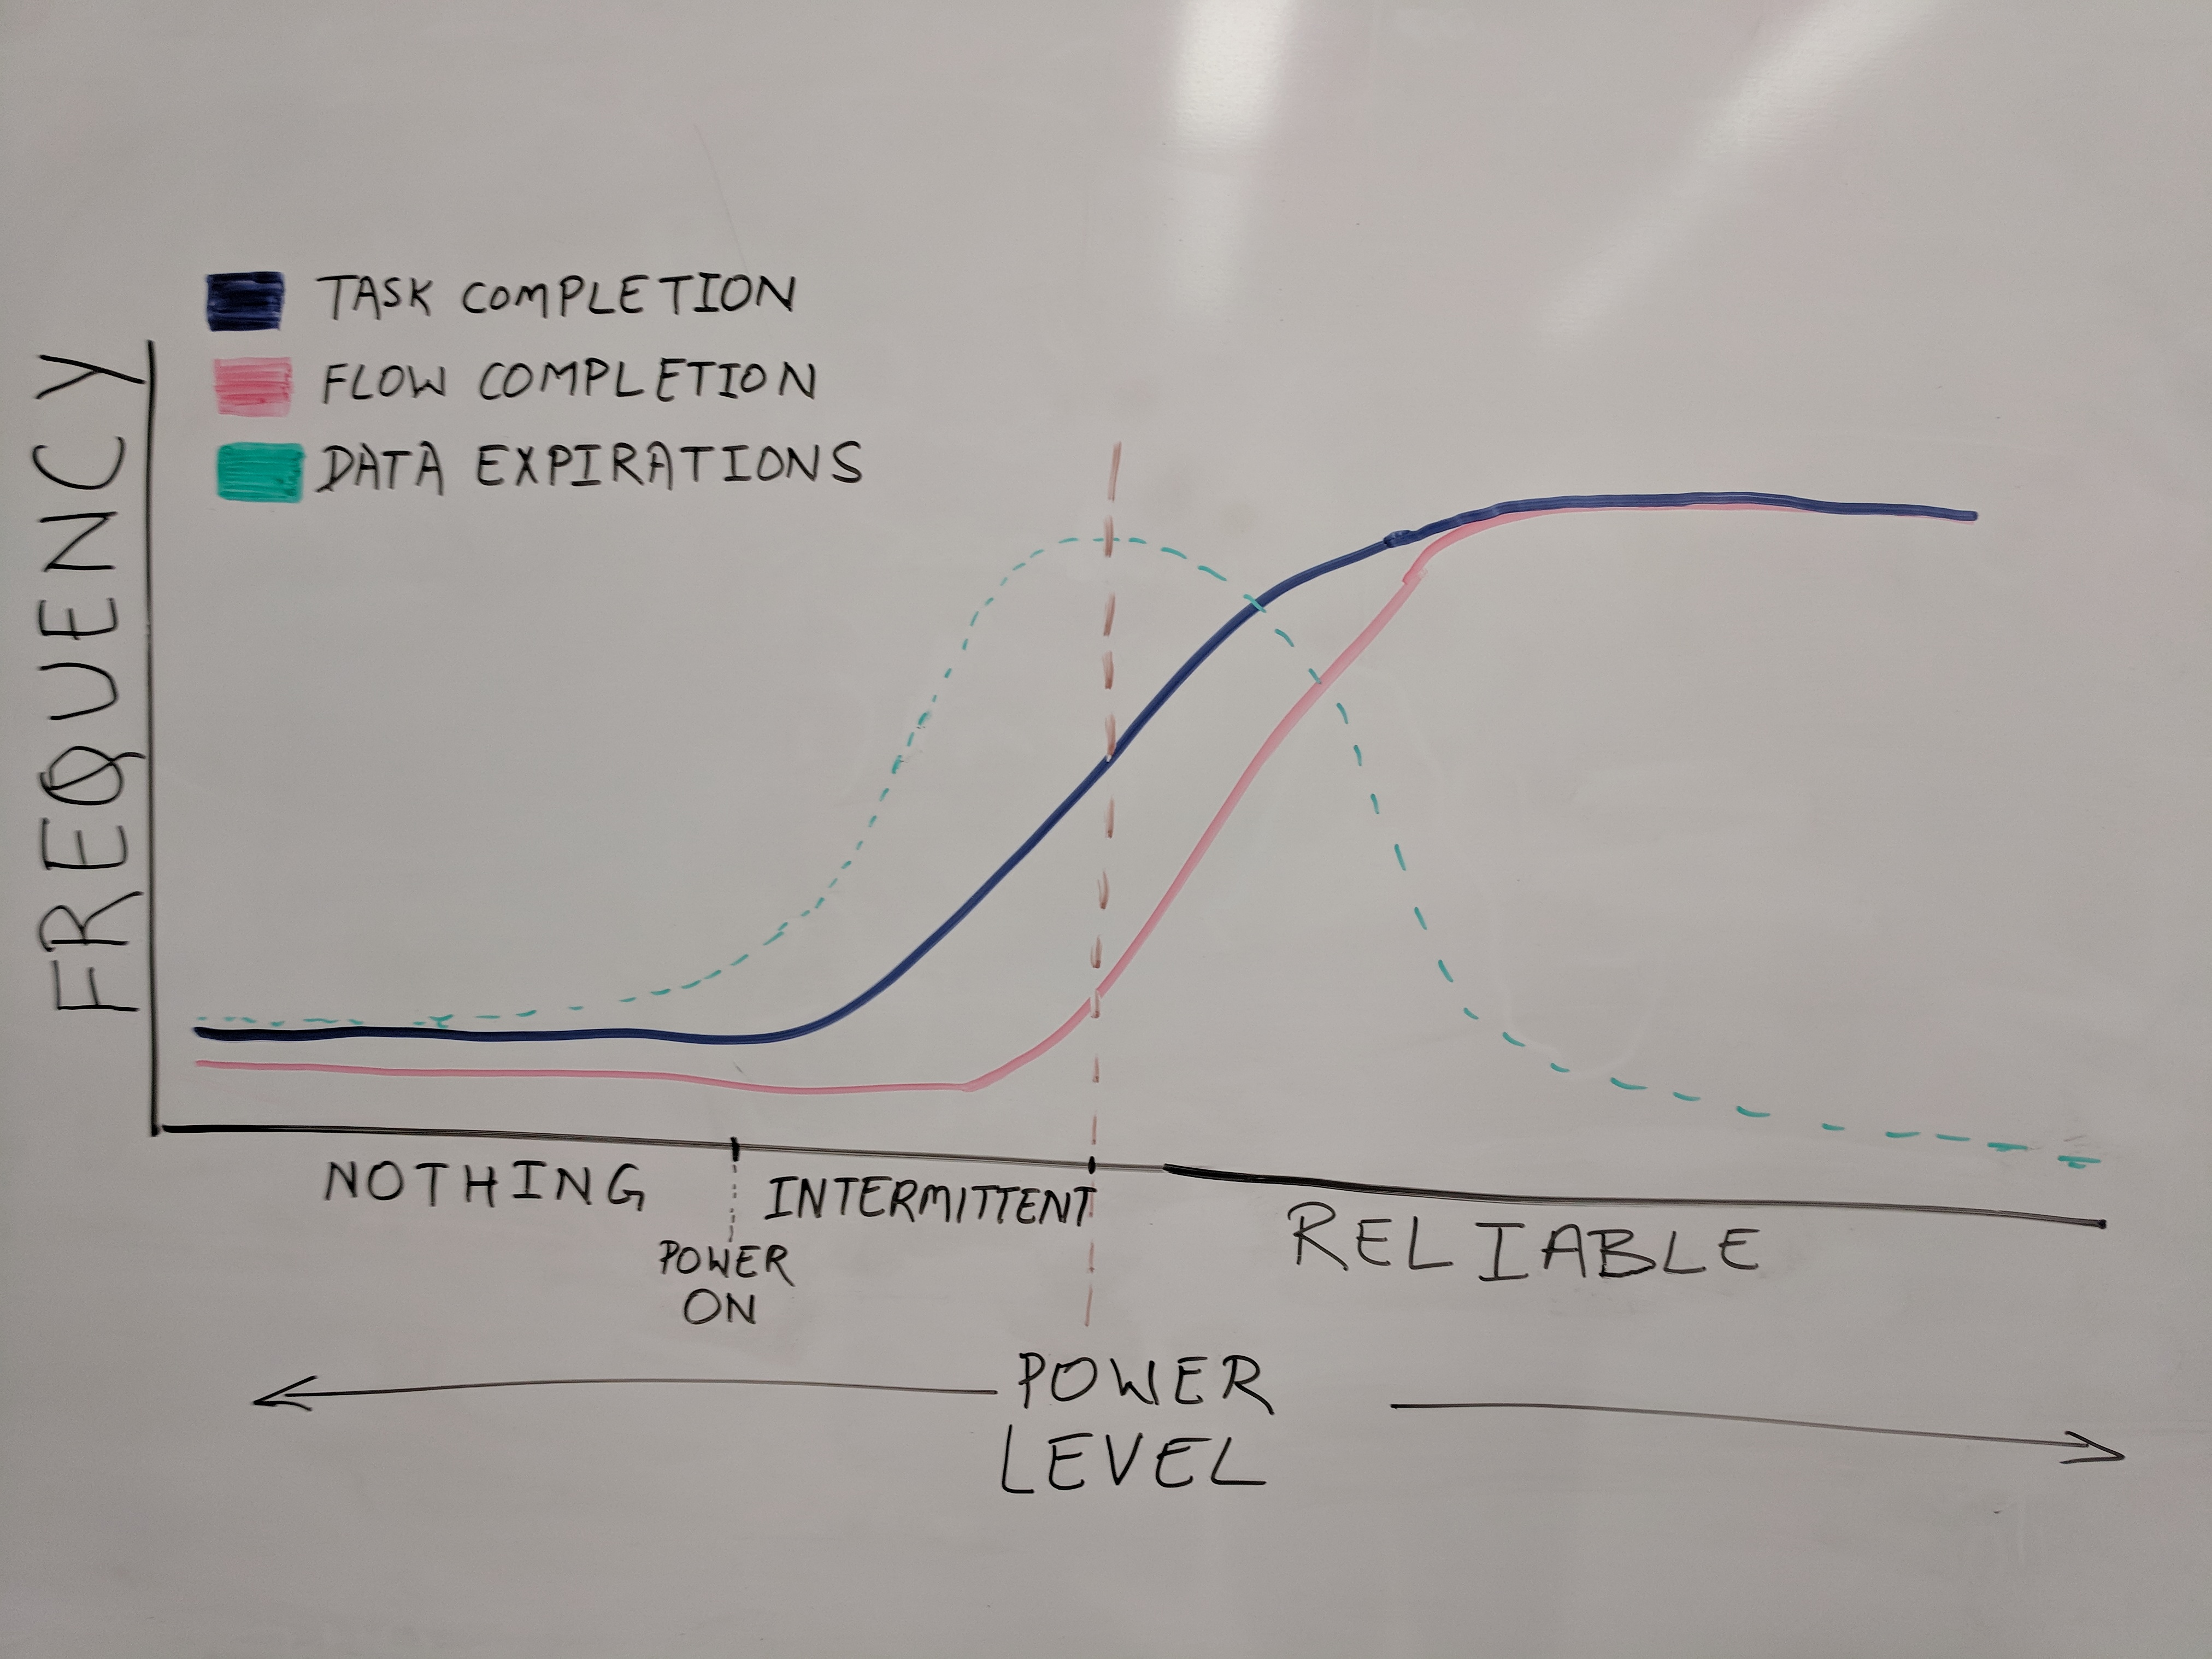
\includegraphics[width=1.0\linewidth]{Figures/graph.jpg}
\caption{
 Graph of data expirations, task and flow completion rate.
}
\label{f:graph}
\end{figure}



\subsection{Work Distribution}

This section details how the work will be distributed between group members.

\subsubsection{Siddhant}
Siddhant's focus on this project is working with the usb powered MSP430.
The data received from the solar launchpad needs to be sent to a laptop computer via serial communication.
Once that channel is working he will use it to send the task and flow completion rates as well as data expirations.
This data will then be used to make the graph shown in Figure \ref{f:graph}.

\subsubsection{Lavaniyaa}
Lavaniyaa's focus on this project is working with the solar powered MSP430.

\subsubsection{Ryan}
Ryan's focus on this project is working with ANTLR to build
Finishing up of ANTLR Task and Flow Identification

\subsection{Completed Goals}

We have designed and submitted a batteryless board for use with the MSP430 to OSHPark, see Figure XXX.
It hasn't arrived yet, but should soon.
In the interim we have been using a more complicated batteryless UFOP board designed by Simeon.
Two simple MSP430 C programs have been written simple sensor reading and simple radio rx/tx.
Since we noticed that everyone was having difficulty with the nRF24L01+ radio we decided to use the cc1101 radio instead.
In addition, we wrote simple code to communicate the task completed to another MSP430.
Two MSP430's are connected via digital pins with the batteryless devices pins set as outputs and the battery powered devices pins set as inputs.
A simple tag grammar for task identification has been written for ANTLR.
Tags will have the following format {\tt |< Task n >|} and |</ Task n >|.
In addition, a simple java program has been written to parse inputted code.
ANTLR works using event handlers that fire when the parser reaches certain code, such as a function definition.

\subsection{In Progress Goals}

Once the boards arrive from OSHPark we will assemble them.
Testing out different solar panel lighting conditions
Send data from MSP to computer for plotting.
Plotting code.
Buildscript for ANTLR + gcc to work as one compiler.
More examples

This model can then be used in combination with the ANTLR compiler to estimate energy usage by the batteryless system.




\subsection{Final Semester Goals}
The final goal of this project is to have multiple energy harvesting systems and applications built.
We plan on having a minimum of two harvesting systems - solar and vibration with two applications each.
We will build our battery based tool that can connect to an energy harvesting system and batteryless device to profile its performance.
The system will be evaluated by comparing the system estimated lifetime with the actual lifetime of the device in a programmable environment, similar to how it was done in Ekho.
